\documentclass[a4paper]{article}
\usepackage{multicol}
\usepackage{url}
\usepackage{graphicx}

\usepackage{amssymb}
\textheight 9.0in
\columnsep 0.375in
\textwidth 6.0in
\footskip 0.0in
\topmargin -0.0625in
\headheight 0.0in
\headsep 0.0in
\oddsidemargin 0.2in 
\parindent 0pc

\pagestyle{empty}
\newtheorem{sample}{Sample}

\begin{document}
\date{}
\title{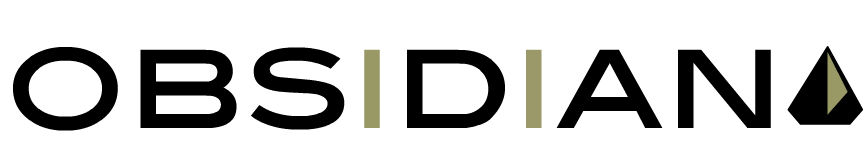
\includegraphics[scale=0.5]{../resources/images/logo_1.png}\textbf{\\}\textbf{\\}\Large \textbf{OBSIDIAN 0.1 DOCUMENTATION
\\}\vspace{0.5cm}}
\author{\textbf{Clement Game}\\clement(at)digi-nation(dot)com}

\maketitle
\thispagestyle{empty}

\vspace{3cm}
\begin{figure}[h]
\begin{center}
\label{fig:orga}
\end{center}
\end{figure}

\clearpage

{\textbf{}
{\small\em }}
\vspace{0.5cm}
{\bf\it \\Keywords:}
{\small Peer-to-Peer,Fast R�plication,mirroring,Dexp,Linux }

\tableofcontents

\textbf{\\ \\ \\ \\}

\thispagestyle{plain}


\section{Introduction}

This is the documentation of the Obsidian Peer-to-Peer mirroring Software,
version 0.1. This paper is released under CC-by-SA licence. \\\\In ancient times, People was using a volcanic stone, which amount of 

\section{Overview}

Obsidian is a fast-mirroring, Peer-to-Peer software which was specially designed to maintain large file repositories synchronized with each others, featuring very fast changes propagating. \\\\To achieve this, Obsidian use 2 core technologies: Filesystem Events Listening , and a new protocol specially designed for the occasion: DEXP, acronym for Documents EXchange Protocol. With DEXP, Change Notifications are sent directly to the mirroring peers, so they don't have to poll periodically for file changes.\\\\

To illustrate how fast is Obsidian compared to a classical multiple rsync-based system, we can do the math:\\\\
Let's consider a chain of n peers, each node being synchronized to the next with a periodical rsynch check $(T_c)$.The time taken by each node to download a change is $T_d$.
In this case, the worst-case propagating time will be:\\\\

$ T_r = \sum_0^n T_d(n) + T_c(n) $\\\\
As we can see in this case (rsync) , the more nodes we have, the more time it loses, because of the accumulation the $T_c$ components.\\\\But in the other case (Obsidian) , the calculation of the maximum propagating time between n nodes is:\\\\
$ T_r  = \sum_0^n T_d(n) $\\\\
So with obisidan, The more nodes you haves, the more efficient it is compared to a periodic-poll based method.If we now consider a $T_c$ constant for each node, we can evaluate the speed gain with: $T_g = nT_c$ \\So the bigger is n, the bigger is the gain.

\section{Global Architecture}

This section explains how Obsidian works from a global point of vew:\\\\

Obsidian nodes are logically grouped by what we call 'Spheres of influence'. Each Obsidian node inside a sphere of influance receive the same announces, 
and all the nodes will end-up hosting the same files database (except if you defined filters, later explained in this document)
 
2 distinct spheres of Influence appear when nobody belonging to sphere 1 has a peering connection to anybody Belonging to sphere 2   

\begin{center}
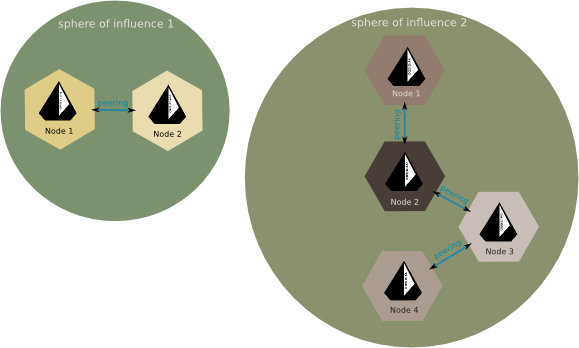
\includegraphics[scale=1]{../resources/images/global_arch_1.png}
\end{center}
Now let's make the model evolve. Node 2 from sphere 1 peers with node 2 from sphere 2: Since These 2 nodes will share announces, the 2 spheres will merge. 

\begin{center}
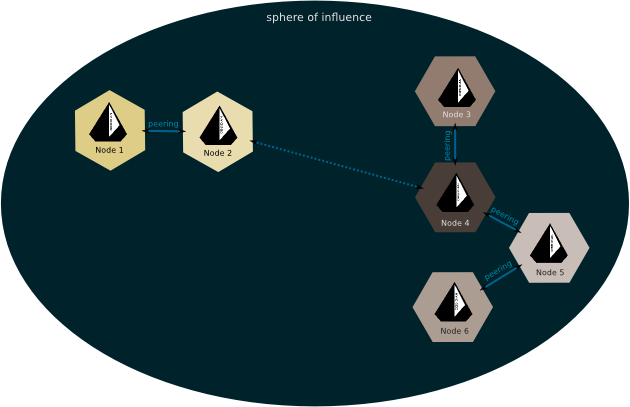
\includegraphics[scale=1]{../resources/images/global_arch_2.png}
\end{center}

$
n1 \epsilon S1 \\
n2 \epsilon S2 \\
peering(n1,n2) =>  n1 \epsilon (S1 \cap S2) , n2 \epsilon (S1 \cap S2)\\\\$



\section{Software Architecture}

The Software architecture behind Obsidian is quite easy, and fit as the following:\\\\

\begin{center}
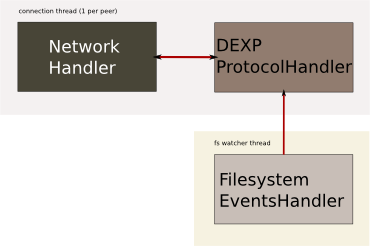
\includegraphics[scale=0.5]{../resources/images/software_arch.png}\end{center}
\section{Getting Started with Obsidian}
This section describes in detail how to get started with Obsidian, step-by-step and from scratch.
\subsection{prerequisites}

In order to build and run Obsidian, you'll need: \\\\

- A GNU/Linux Op�rating System, with kernel 2.6.19 or higher.\\
- The OpenSSL Library plus its headers (libssl-dev) , 0.9.8 or higher.\\
- Cross-platform make (cmake 2.6 or higher).\\
- The GNU C compiler ( gcc-4.X ).\\
- Git DVCS(to retrieve the source code, if not done yet )\\

\subsection{Fetching the sources}

Here we're assuming that that you haven't fetched the obsidian source code yet. To do that, you will need the GIT DVCS, a well-known .

Once you have git installed on your system, just type:\\
 
\verb|git clone git://github.com/digination/obsidian.git |


\subsection{Compilation}

This step explains how to build Obsidian from sources


\subsection{Installation}

To install Obsidian, Nothing is more simple. From the Obsidian Root Directory, just type "make install" , and the Makefile will take care of the rest.

\subsection{Configuration} 

\section{Advanced Usages}

\subsection{Setting up TLS on your obsidian Server}

\subsection{Running multiple sessions of Obsidian on the same server}

In order to circumvence the zero-dir limitation, you can choose to run multiple instances of obsidian at the same time on your server, so your peers can replicate data from the multiple instances.

\section{More on DEXP}

\section{Known Bugs, Limitations}

\section{Special Thanks}


\end{document}